%%%%%%%%%%%%%%%%%%%%%%%%%%%%%%%%%%%%%%%%%
% Wenneker Assignment
% LaTeX Template
% Version 2.0 (12/1/2019)
%
% This template originates from:
% http://www.LaTeXTemplates.com
%
% Authors:
% Vel (vel@LaTeXTemplates.com)
% Frits Wenneker
%
% License:
% CC BY-NC-SA 3.0 (http://creativecommons.org/licenses/by-nc-sa/3.0/)
% 
%%%%%%%%%%%%%%%%%%%%%%%%%%%%%%%%%%%%%%%%%

%----------------------------------------------------------------------------------------
% PACKAGES AND OTHER DOCUMENT CONFIGURATIONS
%----------------------------------------------------------------------------------------

\documentclass[11pt]{scrartcl} % Font size

%%%%%%%%%%%%%%%%%%%%%%%%%%%%%%%%%%%%%%%%%
% Wenneker Assignment
% Structure Specification File
% Version 2.0 (12/1/2019)
%
% This template originates from:
% http://www.LaTeXTemplates.com
%
% Authors:
% Vel (vel@LaTeXTemplates.com)
% Frits Wenneker
%
% License:
% CC BY-NC-SA 3.0 (http://creativecommons.org/licenses/by-nc-sa/3.0/)
% 
%%%%%%%%%%%%%%%%%%%%%%%%%%%%%%%%%%%%%%%%%

%----------------------------------------------------------------------------------------
%	PACKAGES AND OTHER DOCUMENT CONFIGURATIONS
%----------------------------------------------------------------------------------------

\usepackage{amsmath, amsfonts, amsthm} % Math packages

\usepackage{listings} % Code listings, with syntax highlighting

\usepackage[english]{babel} % English language hyphenation

\usepackage{graphicx} % Required for inserting images
\graphicspath{{Figures/}{./}} % Specifies where to look for included images (trailing slash required)

\usepackage{booktabs} % Required for better horizontal rules in tables

\numberwithin{equation}{section} % Number equations within sections (i.e. 1.1, 1.2, 2.1, 2.2 instead of 1, 2, 3, 4)
\numberwithin{figure}{section} % Number figures within sections (i.e. 1.1, 1.2, 2.1, 2.2 instead of 1, 2, 3, 4)
\numberwithin{table}{section} % Number tables within sections (i.e. 1.1, 1.2, 2.1, 2.2 instead of 1, 2, 3, 4)

\setlength\parindent{0pt} % Removes all indentation from paragraphs

\usepackage{enumitem} % Required for list customisation
\setlist{noitemsep} % No spacing between list items

%----------------------------------------------------------------------------------------
%	DOCUMENT MARGINS
%----------------------------------------------------------------------------------------

\usepackage{geometry} % Required for adjusting page dimensions and margins

\geometry{
	paper=a4paper, % Paper size, change to letterpaper for US letter size
	top=2.5cm, % Top margin
	bottom=3cm, % Bottom margin
	left=3cm, % Left margin
	right=3cm, % Right margin
	headheight=0.75cm, % Header height
	footskip=1.5cm, % Space from the bottom margin to the baseline of the footer
	headsep=0.75cm, % Space from the top margin to the baseline of the header
	%showframe, % Uncomment to show how the type block is set on the page
}

%----------------------------------------------------------------------------------------
%	FONTS
%----------------------------------------------------------------------------------------

\usepackage[utf8]{inputenc} % Required for inputting international characters
\usepackage[T1]{fontenc} % Use 8-bit encoding

\usepackage{fourier} % Use the Adobe Utopia font for the document

%----------------------------------------------------------------------------------------
%	SECTION TITLES
%----------------------------------------------------------------------------------------

\usepackage{sectsty} % Allows customising section commands

\sectionfont{\vspace{6pt}\centering\normalfont\scshape} % \section{} styling
\subsectionfont{\normalfont\bfseries} % \subsection{} styling
\subsubsectionfont{\normalfont\itshape} % \subsubsection{} styling
\paragraphfont{\normalfont\scshape} % \paragraph{} styling

%----------------------------------------------------------------------------------------
%	HEADERS AND FOOTERS
%----------------------------------------------------------------------------------------

\usepackage{scrlayer-scrpage} % Required for customising headers and footers

\ohead*{} % Right header
\ihead*{} % Left header
\chead*{} % Centre header

\ofoot*{} % Right footer
\ifoot*{} % Left footer
\cfoot*{\pagemark} % Centre footer
 % Include the file specifying the document structure and custom commands
\usepackage{hyperref} % Include the hyperref package for URLs
\usepackage[backend=bibtex,style=numeric]{biblatex}
\usepackage{csquotes}
\usepackage{algorithm}
\usepackage{algpseudocode}
\addbibresource{Bibliography.bib} % Specify the bibliography file (ensure this file exists and contains entries)


%----------------------------------------------------------------------------------------
% TITLE SECTION
%----------------------------------------------------------------------------------------

\title{	
	\normalfont\normalsize
	\textsc{University of Galway}\\ % Your university, school and/or department name(s)
	\vspace{25pt} % Whitespace
	\rule{\linewidth}{0.5pt}\\ % Thin top horizontal rule
	\vspace{20pt} % Whitespace
	{\huge  Project 1: Evolutionary Search (GAs)}\\ % The assignment title
	\vspace{12pt} % Whitespace
	\rule{\linewidth}{2pt}\\ % Thick bottom horizontal rule
	\vspace{12pt} % Whitespace
}

\author{\LARGE Cathal Lawlor} % Your name

\date{\normalsize\today} % Today's date (\today) or a custom date

\begin{document}

\maketitle % Print the title

\section{Github Repository}
Github repository with code available \href{https://github.com/Laan33/ai_project_1}{here}

\section{Implementation details \& design choices}

\subsection{Tournament Selection}
I used tournament selection for selecting parents for crossover. For my testing, I used a value of 5 for k, as it was a good balance between exploration and exploitation.

As I elaborate on in \ref{Training on all fixed strategies}, for when I wanted to 

\subsection{Crossover method}
I had a uniform crossover method, which used tournament selection to


\subsection{Termination condition}
I implemented a max number of generations to run, but I also added a clause, that if the algorithm hasn't improved by more than 0.25\% in the last 60 generations, it will terminate early.

This is because, genetic algorithms can get stuck in local optima, or just simply converge.

\section{Part 1: Fixed strategies}
\section{Testing}
The agent had a memroy of 2, and only awareness of the enemys moves.

\subsubsection{Training on all fixed strategies}
\label{Training on all fixed strategies}
I trained a generalised agent on all the fixed strategies, with a generalised evaluation function.
I did this as tournament selection would always discount any algorithms who were trained on the \texttt{Always Defect} strategy.
Tournament selection wouldn't picked those agents, even if it was a perfect response to \texttt{Always Defect}, as it results in a really low payout relative to payouts other agents have when faced with 'easier' strategies. 

\begin{figure}[H]
	\centering
	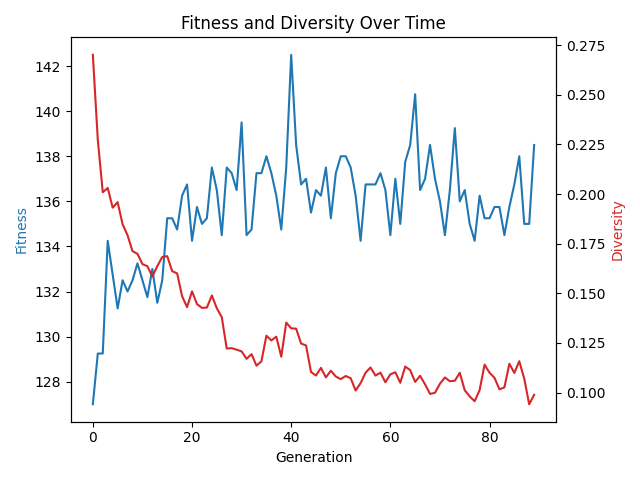
\includegraphics[width=0.8\linewidth]{Figures/part_1/generalised.png}
	\caption{Generalised Trained Alogrithm Tested On All Fixed Strategies}
	\label{fig:general_graph}
\end{figure}

\begin{table}[h!]
    \centering
    \begin{tabular}{|c|c|c|}
        \hline
		\textbf{(Fixed Strategy)} & \textbf{Agent Score} & \textbf{Fixed Strat Score} \\ \hline
        \textbf{Always Cooperate} & 172 & 117\\ \hline
        \textbf{Always Defect} & 50 & 50 \\ \hline
        \textbf{Tit-for-Tat} & 139 & 139 \\ \hline
        \textbf{Adaptive Strategy} & 167 & 122 \\ \hline
        \textbf{Spiteful Strategy} & 120 & 130 \\ \hline
    \end{tabular}
    \caption{Generalised agent performance against each fixed strategy}
    \label{tab:gen_agent_vs_fixed_strats}
\end{table}

With the stopping condition in place, the evolution stopped early at generation 89, as the fitness had plateaued, and the diversity of the population had converged.

As we can see, both in the graph\ref{fig:general_graph} and the results table\ref{tab:gen_agent_vs_fixed_strats}, 
the agent performed well against all the fixed strategies, except for the spiteful and always cooperate strategies.
It isn't a surprise it struggled with the always defect strategy, as the agents training on the adaptive, spiteful and tit-for-tat strategies will have biased it's strategy for when an opponent has played \texttt{CC}. 
We can see this in the table\ref{tab:history_probabilities} representing the probability of the agent complying based on the opponent history.
If the memory was increased, it would almost certainly be able to differentiate the always cooperate strategy from the others.

The agent had a average fitness of 135.71, when averaged over all the fixed strategies 
(which however, isn't normalised for the different max possible results for each strategy), the table above, is a much better representation of the agent's performance.

% The best agent genome representation\ref{tab:history_probabilities} is:
\begin{table}[h!]
	\centering
	\begin{tabular}{|c|c|}
		\hline
		\textbf{(History permutation)} & \textbf{Probability of Cooperate} \\ \hline
		"" & 0.49 \\ \hline
		C & 0.86 \\ \hline
		D & 0.11 \\ \hline
		CC & 0.74 \\ \hline
		CD & 0.94 \\ \hline
		DC & 1.0 \\ \hline
		DD & 0.0 \\ \hline
	\end{tabular}
	\caption{Best generalised agent strategy genome}
	\label{tab:history_probabilities}
\end{table}

\subsubsection{Specific agents against other fixed strategies}

For fun, for each fixed strategy, I trained an agent against only that specific strategy, and then had the best evolved agent play all of the other strategies.

Some notable results: unsurprisingly, the \texttt{Always Cooperate} strategy performed well when it was tested against itself and the and \texttt{Always Defect} strategy, as it always was going to select the highest reward option, being always defect.
It did hold it's own though against the two other strategies, came out on top against the other three strategies.

The \texttt{Always Defect} strategy performed the worst, as it only knew what to do when the other agent defected twice in a row. 
The only wins it had were when the other combinations were used and it happened to have a random value initialised that proved to be lucky.


The adaptive and tit for tat strategies are interesting to look at in how they performed.
\texttt{Tit-for-Tat} was quite compliant, and matched equal scores, except for when it was confused by \texttt{Always Defect} (as it not had any training experience with repeated \texttt{DD}).
\texttt{Adaptive Strategy} did well with \texttt{Always Cooperate}, but lost miserably out to \texttt{Always Defect}. Otherwise, it matched well for the other two tests.

% Agent Score / Fixed Strategy Score
% \subsubsection{Against other strategies}
% \begin{table}[h!]
%     \centering
%     \begin{tabular}{|c|c|c|c|c|c|}
%         \hline
% 		\textbf{(Trained On)} & \multicolumn{5}{c|}{\textbf{Fixed Strategy (Tested On)}} \\ \hline
%         \textbf{} & \textbf{Always Cooperate} & \textbf{Always Defect} & \textbf{Tit-for-Tat} & \textbf{Adaptive Strategy} & \textbf{Sum of Score} \\ \hline        
%         \textbf{Always Cooperate} & 250 / 0 & 49 / 54 & 114 / 109 & 61 / 51 & 469\\ \hline
%         \textbf{Always Defect} & 166 / 126 & 50 / 50 & 54 / 49 & 60 / 55 & 325\\ \hline
%         \textbf{Tit-for-Tat} & 150 / 150 & 10 / 210 & 150 / 150 & 150 / 150 & 460\\ \hline
%         \textbf{Adaptive Strategy} & 176 / 111 & 2 / 242 & 131 / 131 & 151 / 131 & 460\\ \hline
%     \end{tabular}
%     \caption{Agent performance against fixed strategies after training on different opponents}
%     \label{tab:agent_vs_fixed_strats}
% \end{table}




% \begin{figure}[h!]
% 	\centering
% 	\includegraphics[width=0.8\linewidth]{convergence_example_.png}
% 	\caption{Example of convergence over generations}
% 	\label{fig:convergence_example}
% \end{figure}
%------------------------------------------------

\section{Part 2: Extension}

\textbf{Disclaimer:} 
I didn't read the assignment spec initially and actually made a much more complex genome for part 1, and actually didn't have too much to extend for part 2. (I had a memory of 2, and probabilities rather than binary decisions)
Here is what I have changed:
\begin{itemize}
	\item Increased memory from 2 to 6.
	\item Added noise.
	\item 
\end{itemize}

\subsubsection{Experimentation setup}
To evaluate the performance of the genetic algorithm (GA) for the travelling salesperson problem (TSP), I ran experiments on three different datasets: berlin52, kroA100, and pr1002.


\subsubsection{Best crossover method}

\subsubsection{Best mutation method}
n 
\subsubsection{Best parameters}

\section{Comparison with known optimal solutions}
\label{Comparison with known optimal solutions}



\section{Potential improvements}
\label{Potential improvements}




% One easy, improvment I believe for my algorithm would be to employ elitism.
% I implemented it in a early version of the program. I chose not to implement it, as I wanted to see how the various methods for crossover and mutation would handle the problem alone, without the help of elitism.
% It would probably extract a small bit more performance out, especially for the bigger datasets, less so in the Berlin dataset.

% I believe that tournament selection is a good choice, being the sweet spot for a genetic algorithm solving TSP. It's fast, simple, and maintains a good diversity and doesn't suffer with early convergence like roulette wheel selection can\cite{genetic_algorithm_afternoon}.
% I also tried monte carlo selection, but I do not believe it works for the travelling salesperson problem.

% Another, is to run the same parameters multiple times on differening starting populations, and averaging the results. This would give a more accurate representation of the algorithm's performance, as the starting population can have a big impact on the final result. e.g. it may get stuck in a local optima, or converge too early.
% Also related to this, is to allow the algorithm to do hyperparameter tuning on the fly (e.g. using adaptive mutation or crossover rates based on fitness), as it's running. This would allow the algorithm to adjust to the problem, and the population, as it's running, and not just at the start.

% For the bigger pr1002 dataset, I think given more time and resources would help improve the results on the large pr1002 dataset. 
% Mainly, this would allow me to up the population size by a lot, which then allows it to run for a lot more generations without converging too early, allowing more exploraiton of the solution space.

% There is other improvements, such as a hybrid approach of a local search algorithm, e.g. 2-opt, to improve the final solution once the genetic algorithm has converged. This would help fine-tune the solution, and get a better result.

\printbibliography
\end{document}
